\documentclass{../template/llncs}
%
\usepackage{url}
\RequirePackage[hyphenbreaks]{breakurl} % allow hyphenation in URLs
\usepackage{amsmath} % use equations
\RequirePackage[utf8]{inputenc} % support Umlauts and special characters
\usepackage{microtype} % use space more efficiently and hyphenate smarter: all in all looks a lot sexier
\usepackage{listings} % allow source code environments
% Define a listing style for FLUX code
\lstdefinestyle{flux} {
  frame=L,
  xleftmargin=\parindent,
  basicstyle=\footnotesize\ttfamily,
  breakatwhitespace=true,
  numbers=left,
  escapechar=\%,
  numberstyle=\tiny,
  numberblanklines=false,
  captionpos=b,
  emph={perform, poss, state\_update, main\_loop, init},
  emphstyle=\textbf,
}
%
\title{Logic Programming}
\subtitle{Introducing GOLOG and FLUX}
\titlerunning{logprog}
\author{Michael Ruster}
\institute{University Koblenz-Landau}
\tocauthor{ }
%
\begin{document}
\maketitle
\tableofcontents

\section{Introduction}
Deploying of autonomous agents becoming more and more important nowadays. Agents act in complex production environments, where failure of a single agent may cause serious losses. The challenge for multi-agent systems now is how to make sure that the agent will not behave unacceptable or undesirable? Formal methods had been used in computer science as a basis to solve correctness challenges. They represent agents as a high level abstractions in complex systems. Such representation can lead to simpler techniques for design and development.

There are two roles of formal methods in distributed artificial intelligence that are often referred to. Firstly, with respect to precise specifications they help in debugging specifications and in validation of system implementations. Abstracting from specific implementation leads to better understanding of the design of the system being developed. Secondly, in the long run formal methods help in developing a clearer understanding of problems and their solutions. \cite{Singh_99}

This report in the first section will cover very briefly the theoretical background consisting of different types of logics and introduced operators. Later we will discuss formal methods for a single autonomous agent and the basic implementation of the interpreter. Next some concepts for multiple communicating agents will be introduced. And, finally, the report will conclude with a brief summary of the discussed topic. 

\section{Situation Calculus}\label{sitCalc}
The situation calculus was introduced by McCarthy and Hayes~\cite{mccarthy_philosophical_1969}. It is mainly a fist-order logic but also encodes a dynamic world through second order logic \cite{levesque_golog:_1997}. The situation calculus consists of the three first-order terms \emph{fluents}, \emph{actions} and \emph{situations}. Fluents model properties of the world. Actions may change fluents and hence may modify the world. Every action is ``logged'' in the situation. Therefore, a situation is a history of actions up to a certain point in time starting from the initial situation $s_0$. Due to the initial situation modelling the situation before any action has been executed, there can only be one initial situation.

Fluents can be evaluated to return a result. As they are situation dependent, the evaluation result may change over time. Fluents are distinguished in \emph{relational fluents} and \emph{functional fluents}. Relational fluents can hold in situations. Their evaluation hence may return either true or false. An example is given in (\ref{f_hasCoffee}) with $p$ being an agent and $s$ a situation.
\begin{equation}\label{f_hasCoffee}
  \textit{hasCoffee}(p,s)
\end{equation}
Functional fluents return values instead. A fluent $\textit{location}(p,s)$ may return the coordinates $(x,y)$ as an example.

Actions also depend on situations. The reason for this is that actions might not always be executable. Instead, it is possible that certain actions need specific fluents to hold which are modified by actions. Describing when an action is executable is done with \emph{action precondition axioms}. This is expressed by the predicate $\textit{Poss}(a,s)$ with $a$ being an action. As a recurring example, let us think of the ability to pour coffee to an agent $p$. This must only be possible when $p$ does not already have coffee. Equation~(\ref{a_possPourCoffee}) illustrates how this can be formalised.
\begin{equation}\label{a_possPourCoffee}
  \textit{Poss}(\textit{pourCoffee}(p),s) \Leftrightarrow \neg \textit{hasCoffee}(p,s)
\end{equation}

As mentioned before, the execution of action must always alter the situation: $\textit{do}(a,s) \rightarrow s'$. Its effects on the world say fluents are described with \emph{action effect axioms}. Equation~(\ref{a_effectPourCoffee}) shows how pouring a coffee to $p$ will result in $p$ having coffee afterwards.
\begin{equation}\label{a_effectPourCoffee}
  \textit{Poss}(\textit{pourCoffee}(p),s) \rightarrow \textit{hasCoffee}\big(p,\textit{do}(\textit{pourCoffee}(p),s)\big)
\end{equation}
In (\ref{a_effectPourCoffee}), it is unclear whether other fluents stay unaffected. For example, reasoning about $location(p,s')$ would not be possible, with $\textit{do}(\textit{pourCoffee}(p,s)) \rightarrow s'$. With this arises the so called called \emph{frame problem}. Defining for every fluent how every action may or may not affect is only a theoretical solution. The reason for that is that the resulting complexity of $\mathcal{O}(A*F)$ would be too high even in most small worlds. A feasible solution to this problem was proposed by Reiter~\cite{reiter_frame_1991}. His approach was to define every effect of allactions only once. Thus Reiter reduced the complexity to $\mathcal{O}(A*E)$. This solution is known as the \emph{successor state axiom} shown in (\ref{sucStateAxiom}).
\begin{equation}\label{sucStateAxiom}
  \mathit{Poss}(a,s)\rightarrow \big[\mathit{F}(\mathit{do}(a,s)) \Leftrightarrow\gamma_\mathit{F}^+(a,s)\vee\mathit{F}(s)\wedge\neg\gamma_\mathit{F}^-(a,s)\big]
\end{equation}
$\mathit{F}(\mathit{do}(a,s))$ means that the fluent $F$ will be true after exectuing the action $a$. The first part of the disjunction is $\gamma_\mathit{F}^+(a,s)$ and expresses that the action made the fluent true. $\mathit{F}(s)\wedge\neg\gamma_\mathit{F}^-(a,s)$ as the second part expresses that the fluent had been true before and the action had no influence on it. For a reasonable example, there needs to be a second action which does not influence (\ref{f_hasCoffee}). Therefore, the $sing(s)$ action will be introduced which has no effect on any fluents and can be executed anytime as shown in (\ref{a_possSing}).
\begin{equation}\label{a_possSing}
  \mathit{Poss}(\mathit{sing}) \Leftrightarrow \top
\end{equation}
Given (\ref{f_hasCoffee}), (\ref{a_possPourCoffee}) and (\ref{a_possSing}) an example can be compiled like in (\ref{a_sucStateAxiom}):
\begin{equation}\label{a_sucStateAxiom}
  \begin{split}
    \mathrm{Poss}(a,s)\rightarrow \big[&\mathrm{hasCoffee}(p,\mathrm{do}(a,s))
\\    &\Leftrightarrow [a=\mathrm{pourCoffee}(p)]
\\    &\vee\ [\mathrm{hasCoffee}(p,s) \wedge a\neq \mathrm{pourCoffee}(p)]\big]
  \end{split}
\end{equation}
Equation (\ref{a_sucStateAxiom}) then formalises that an agent $p$ may only have coffee if it was poured coffee or if it already had coffee and the action was not to pour $p$ a coffee.


\section{GOLOG}\label{golog}
GOLOG is a language for logic programming introduced by Levesque et~al.~\cite{levesque_golog:_1997}. It builds on the situation calculus. To allow high-level programming, GOLOG adds complex actions like loops, conditions, tests and non-deterministic elements. As an example, a GOLOG program should have a robot pouring other agents coffee until everybody does have coffee. After that, the robot should sing and terminate. Such a program would reuse the fluent in (\ref{f_hasCoffee}), the action precondition axioms in (\ref{a_possPourCoffee}), (\ref{a_possSing}), the successor state axiom in (\ref{a_sucStateAxiom}) and extend them with the two procedures given in (\ref{p_control}) and (\ref{p_pourSOCoffee}):
\begin{equation}\label{p_control}
  \begin{split}
    \textbf{proc}\ \texttt{control}\ [&\textbf{while}\ (\exists p) \neg\textit{hasCoffee}(p) \\
    &\textbf{do}\ \texttt{pourSOCoffee}(p)\ \textbf{endWhile}]; \\
    \textit{sing}&\ \textbf{endProc}.
  \end{split}
\end{equation}
\begin{equation}\label{p_pourSOCoffee}
  \begin{split}
    \textbf{proc}\ \texttt{pourSOCoffee}\ (\boldsymbol{\pi} p)\ [ &\neg\textit{hasCoffee}(p)\textbf{?}; \\
    &\textit{pourCoffee}(p)]\ \textbf{endProc}.
  \end{split}
\end{equation}
The control procedure in (\ref{p_control}) can be seen as a main method. It loops as long as there exist agents without coffee and tells the robot to pour coffee to some agent lacking coffee. In the end, the robot sings. Equation (\ref{p_pourSOCoffee}) allows the robot to non-deterministically choose an agent $p$ to pour coffee to by using the $\pi$-operator. The $?$-operator is similar to the \texttt{if}-operator in other programming languages like Java. Due to the non-determinsmic operator, there can be two different resulting situations like shown in (\ref{ex_situations}) with the initial configuration given in (\ref{ex_gologConfiguration}):
\begin{equation}\label{ex_gologConfiguration}
  \neg\textit{hasCoffee}(p,s_0) \Leftrightarrow p=\textrm{Miriam} \vee p=\textrm{Sergey}.
\end{equation}
\begin{equation}\label{ex_situations}
  \begin{split}
    s=\textit{do}\Big(\textit{sing},\textit{do}\big(&\textit{pourCoffee}(\textrm{Miriam}),
      \textit{do}(\textit{pourCoffee}(\textrm{Sergey}),s_0)\big)\Big),
\\  s=\textit{do}\Big(\textit{sing},\textit{do}\big(&\textit{pourCoffee}(\textrm{Sergey}),
      \textit{do}(\textit{pourCoffee}(\textrm{Miriam}),s_0)\big)\Big)
  \end{split}
\end{equation}

Levesque et~al.~\cite{levesque_golog:_1997} highlight some problems with GOLOG. These make it unsuitable for a multiple agent-based scenario like the Mars-scenario of the MAPC\footnote{\url{https://multiagentcontest.org/}, online -- last accessed 01.05.2014, 16:00.} without considerable modifications and extensions. One problem is that complete knowledge is assumed in the initial situation. This is obviously not the case for scenarios with unknown worlds that get explored by agents. The second problem is that GOLOG does neither offer a solution for internal nor external reactions of agents on sensed actions. A third problem is that exogenous actions say actions out of the agent's control cannot be handled. These could e.g. be actions in control of nature like sudden rain, which are assumed not to be caused by an agent. A fourth problem is highlighted by Thielscher~\cite{thielscher_flux:_2005} and arises from GOLOG being \emph{regression-based}. This means that for deciding whether an action is executable is only possible after looking at all previous actions and how they might have affected the world. As a result, reasoning takes exponentially longer over time and hence GOLOG does not scale.


\section{FLUX}\label{flux}
\lstset{style=flux} % activate flux syntax highlighting in listings
FLUX was introduced by Thielscher~\cite{thielscher_flux:_2005} and offers solutions for the problems of GOLOG presented before. This is done by using the \emph{fluent calculus} instead of the situation calculus. Both are similar but the fluent calculus adds \emph{states}. A state $z$ is a set of fluents $f_1,\cdots,f_n$. In FLUX, it is denoted as $z = f_1 \circ \ldots \circ f_n$. In every situation there always exists only one state with which the current properties of the world are described. Yet, the world can be in the same state in multiple situations. For representing agent knowledge which can be incomplete, FLUX uses \emph{knowledge state}. These are denoted through $\textit{KState}(s,z)$ meaning that an agent knows that $z$ holds in $s$.

The frame problem is solved through \emph{state update axioms}~\cite{thielscher_situation_1999}. They define the effects of an action as the difference between the state before and after the action. This is modelled with $\vartheta^-$ for negative and $\vartheta^+$ for positive effects. Both are simply macros for finite states. Due to using states, reasoning is linear in the size of the state representation. This is called being \emph{regression-based} and therefore FLUX can outperform GOLOG \cite{thielscher_flux:_2005}.

Disjunctive and negative state knowledge is modelled through constraints. FLUX uses a constraint solver To simplify these constraints until they are solvable. This is done by using \emph{constraint handling rules} introduced by Frühwirth~\cite{fruhwirth_theory_1998}. Their general form is shown in (\ref{chr}). It consists of one or multiple heads $H_m$, zero or more guards $G_k$ and one or multiple bodies $B_n$.
\begin{equation}\label{chr}
  H_1,\ldots,H_m\Leftrightarrow G_1,\ldots,G_k \mid B_1,\ldots,B_n
\end{equation}
The general mechanism is that if the guard can be derived, parts of the constraint matching the head will be replaced by the body and hence get simplified. This constraint solver builds the kernel say the foundation of FLUX programs. The domain encodings are built on top of this. Included are the initial knowledge state(s), domain constraints, as well as the action precondition and state update axioms. The final part of a FLUX program is the programmer defined intended agent behaviour called strategy. As a trivial example program, the previous example implemented in GOLOG will be transferred to FLUX in Prolog:
\begin{lstlisting}[caption={Defintion of the \texttt{sing}-action.}, label=lst_sing]
  perform(sing, []).
  poss(sing, Z) :- all_holds(hasCoffee(_), Z).%\label{l_possSing}%
  state_update(Z, sing, Z, []).%\label{l_supSing}%
\end{lstlisting}
Listing~\ref{lst_sing} shows the definition of the \texttt{sing}-action. Empty arrays could be replaced by sensed information that could then effect the outcome of the methods. As this is a trivial example, no sensed information is assumed. Line~\ref{l_possSing} is the precondition that singing is only possible in a state where every agent has coffee. As singing should not alter any fluents, the state \texttt{Z} in line~\ref{l_supSing} is not modified and returned as \texttt{Z}.
\begin{lstlisting}[firstnumber=4, caption={Definition of the \texttt{pourCoffee}-action}, label=lst_pourCoffee]
  perform(pourCoffee(P), []).
  poss(pourCoffee(P), Z) :-
       member(P,[miriam,sergey]),%\label{l_memberP}%
       not_holds(hasCoffee(P), Z).
  state_update(Z1, pourCoffee(P), Z2, []) :-
       update(Z1, [hasCoffee(P)], [], Z2).%\label{l_updateZ}%
\end{lstlisting}
In Listing~\ref{lst_pourCoffee} the \texttt{pourCoffee}-action is defined similarly. Line~\ref{l_memberP} ensures that Prolog will only look for agents that actually exist instead of iterating over memory addresses. The action must modify the state by adding \texttt{hasCoffee(P)} to the state as it is done in line~\ref{l_updateZ}. The empty array after it corresponds to $\vartheta^-$, which is empty in this case.
\begin{lstlisting}[firstnumber=10, caption={Main method which either tells the robot to sing or to pour coffee.}, label=lst_main]
  main_loop(Z) :-
    poss(sing, Z)
      -> execute(sing, Z, Z);
    poss(pourCoffee(P), Z)
      -> execute(pourCoffee(P), Z, Z1),
         main_loop(Z1);
    false.%\label{l_false}%
\end{lstlisting}
Listing~\ref{lst_main} models the main method and thus is similar to (\ref{p_control}). When singing is possible, the robot will do so and terminate. Else, it will pour someone a coffee and call the main loop again. Line~\ref{l_false} ensures that Prolog will return \texttt{No} if neither of the both actions get triggered at some point.
\begin{lstlisting}[firstnumber=17, caption={Initial configuration.}, label=lst_init]
  init(Z0) :-
         not_holds(hasCoffee(miriam), Z0),
         not_holds(hasCoffee(sergey), Z0).
\end{lstlisting}
The initial configuration in listing~\ref{lst_init} is comparable to (\ref{ex_gologConfiguration}) but due to Prolog interpreting from top to bottom, the result will only be \texttt{Z = [hasCoffee(sergey), hasCoffee(miriam)]}.


\section{Conclusion}\label{conclusion}
In this last part, we reflect on the actual competition as well as our own work.
First, \autoref{con:competition} presents the setup and procedure of the competition, as well as the results.
Moreover, some general observations we made while monitoring the behaviour of our agents throughout the matches are given in this section.
\autoref{con:learned} builds upon these observations by explaining in more detail the things we noticed and the conclusions we were able to draw from them.
This section also discusses more general lessons we have learned while developing our multi-agent system.

\subsection{Competition results$^{\odot,\circ}$} % TODO for now, the comma should indicate that this text has been written by @manuelmittler and has only gotten smaller updates/corrections from @0nse.
The competition took place on two dates (15th and 17th of September) and each team had to play three simulations against all other teams.
Every simulation consisted of a total of 400 steps.
The team with the higher overall score at the end received three points for their victory.
Said overall score is the sum of all 400 step scores.
The score per step is composed of points for zones plus achievement points.
Since the strategy of team MAKo was to extensively buy upgrades for the so-called artillery agent, most of the earned achievement points were consumed and therefore did not count towards the step score.
\autoref{dis:achievement_points} shows the progress of achievement points over time.
As can be seen, the achievement points of team MAKo go up and down due to the buying actions whereas the the points of the other team increase constantly.
\begin{figure}[ht]
	\centering
	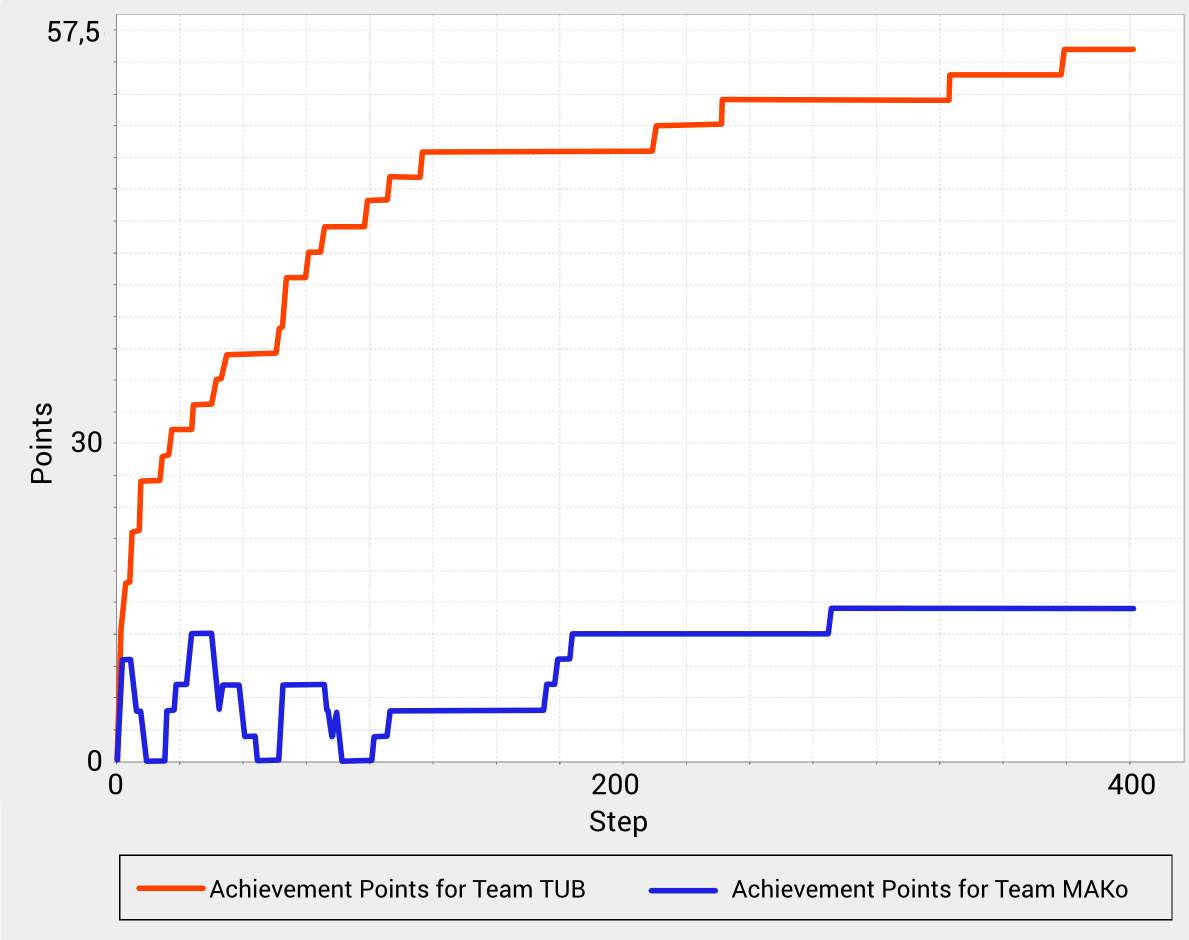
\includegraphics[width=0.7\textwidth]{images/AchievementPoints.png}
	\caption{Achievement points from the second match TUB against MAKo.} % TODO I just wrote second as a filler. What match was it?
	\label{dis:achievement_points}
\end{figure}
On first sight, one could assume that this strategy was a drawback because achievement points earned at some point count into every future step score.
But compared to the number of points awarded for zones, the achievement points are only a minor fraction of the step score.
As it can be seen in \autoref{dis:ZonesScoresAndAchievementPoints} the spending of achievement points did not interfere dramatically with the overall score.
It was worth spending the achievement points for the purpose of attacking and disturbing the other team.
This was because the amount of potential zone points they would have earned without being attacked, would probably have been much higher than the amount of achievement points team MAKo spent for upgrades.
\begin{figure}[h]
	\centering
	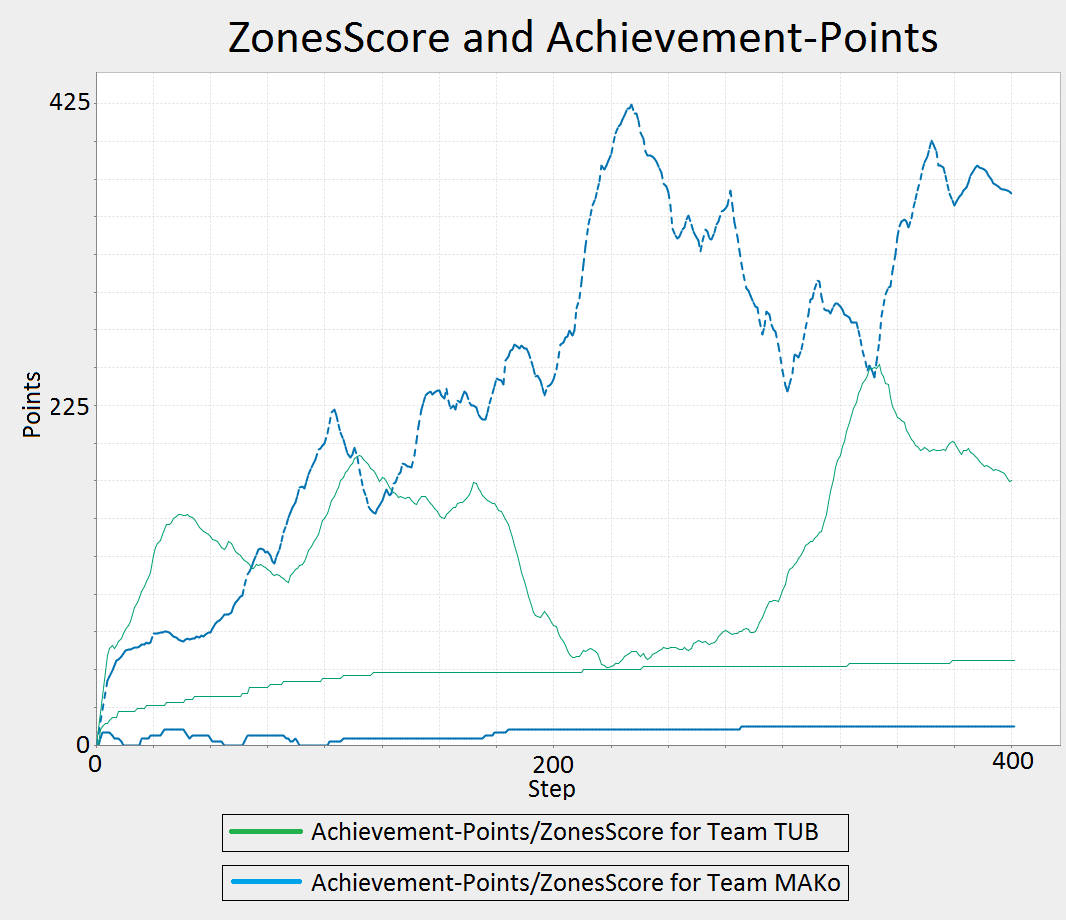
\includegraphics[width=0.7\textwidth]{images/ZonesScoresAndAchievementPoints.png}
	\caption{Combined achievement and zone scores from the second match TUB against MAKo.} % TODO I just wrote second as a filler. What match was it?
	\label{dis:ZonesScoresAndAchievementPoints}
\end{figure}
At the end of the tournament team MAKo scored second with a total of 18 points.
The winner of 2014 was, for the third time in a row, the team from the Federal University of Santa Catarina (UFSC).
The final results are shown in~\autoref{tab:mapc2014results}.
\begin{table}[ht]
  \centering
  \begin{tabularx}{\textwidth}{| l | X | p{2cm} | X | p{2cm} | l |}
    \hline
    \textbf{Pos.} & \textbf{Team name} & \textbf{Country} & \textbf{Score}       & \textbf{Difference} & \textbf{Points} \\ \hline
    1             & SMADAS-UFSC        & Brazil           & 1180662 : 654624     & \ 526038            & 33              \\
    2             & MAKo               & Germany          & \ \ 617086 : 776868  & -15782              & 18              \\
    3             & TUB                & Germany          & \ \ 904874 : 872399  & \ 32475             & 15              \\
    4             & TheWonderbolts     & Denmark          & \ \ 711001 : 1014669 & -303668             & 15              \\
    5             & GOAL-DTU           & Denmark          & \ \ 653178 : 748241  & -95063              & 9               \\ \hline
    % \phantom will generate a newline for some reason so I had to replace it with \
  \end{tabularx}
  \caption{The results of the 2014 MAPC. Each team played three matches against every other team, and winning a match awarded 3 points.}
  \label{tab:mapc2014results}
\end{table}
Statistics of all the individual games can be found in the appendix.[reference here!!!!] % TODO I'm unsure what all you want to add here. But I'll just add this todo here so that we can grep for TODOs in the document itself :)

Our team MAKo lost every second game against all opponents.
This was due to the repairer agents not being able to repair.
We were unable to figure out why this problem arose.
But we found out that manually restarting our agents solved the problem.
Unfortunately as a result, the knowledge about the graph acquired by the agents prior to restarting was reset.
Consequently, the agents surveyed and probed redundantly.
This behaviour was especially surprising as our agents fully restarted automatically after each round and there were no such problems in all third rounds.
The restarts were all manually supervised and showed no sign of failure at any time.

Disregarding this problem, our matches can be summarised as the follows.
Our agents successfully explored the map, repaired disabled agents and attacked the opponent.
Once our designated artillery agent had stopped upgrading, it did not have to move much anymore.
Instead, it effectively attacked distant enemies and recharged mainly to attack afterwards again.
This and the other saboteur agents which were always in search for enemy agents to attack helped disturb the zone building of the other teams.
First, disabled agents were not able to build zones.
Second, disabled agents needed to be repaired which could make the repairer agents temporarily unusable for zoning depending on the strategy the enemies implemented.
If the enemy repairer agents moved towards disabled agents, they could break up a zone which they had been in earlier.

While monitoring the competition, we saw that zoning was subpar.
Due to the fact that zones were broken up periodically, zones with a high value were sometimes discarded even when there was no need to.
Furthermore, the asynchronous communication during zone finding did not work as well as hoped for.
This was partly related to our agents being attacked and disabled by enemy agents.
Agents which ought to form a zone unpredictably had to cancel their zoning availability and get repaired.
Also, we did not implement an algorithm to detect the ``end'' of the graph, say the edges of the map.
% TODO: I'm not happy to talk about grpah ``ends''. Anybody has a suggestion for a better term?
In the course of the matches, we saw that multiple maps favoured such an approach.
\autoref{dis:edgeCases} shows the top left part of the graph from the third match of MAKo against GOAL-DTU.
A single well-placed agent, here depicted as a green rectangle, could in this case create a zone over 25 vertices.
Being able to detect these graph ``ends'' would have enabled us to form greater zones with fewer agents than what our algorithm calculated.
\begin{figure}[h]
	\centering
	
\includegraphics[width=0.5\textwidth]{images/resultsEdgeCase.eps}
	\caption{One agent alone forming a zone over 25 vertices by exploiting the graph ``ends''.}
	\label{dis:edgeCases}
\end{figure}
Nevertheless, the general idea regarding small zone forming proved to be a good choice.
One big zone would have been easy to disturb.
But having multiple small high value zones was quite effective in not providing the enemy with an easy target.

All in all, we are content with the results.
Considering the short time we had until the competition without prior knowledge in this field, we managed to rank second.
This is especially acceptable as the winning team won for the third time in a row and was only beat once due to technical problems.


\subsection{Lessons learned$^\odot$}
None of the "MaKo" team member had experience with Jason as a programming language before the research lab. The first thing that caused problems was that Jason was quite slow, especially when it comes to communication between agents. Since agents most times needed some information from others and could not continue with their reasoning until this information was given, communication was a extreme bottleneck. Extreme delay was observed when the group tried to exchange information about the graph. The first approach was to communicate everything that an agent perceives, while exploring the graph, to every other agent. The reason behind this was to have every agent store the full knowledge about the until then explored (sub-)graph. This course of action was quickly discarded, because agents were not able to do actions while processing all the incoming messages. The next attempt to reduce communication was to implement a so called "cartographer" agent. The purpose of this agent was to have an additionally agent in the background that gathers all the information about the map that all 28 agents perceive. With that cartographer agent the amount of communication was reduced and agents could act like intended, because now they just sent their percepts to the cartographer agent and they had not to deal with incoming messages of the other 27 agents. The drawback of this approach revealed when it came to querying the cartographer agent for information, for instance when an agent wanted to know if a vertex was already surveyed or how he could reach given vertex. Like it was noticed before, processing the received messages is quite slow and so it happened that the cartographer agent was not able to handle messages in time. It occurred that agents asked about some specific vertex which the cartographer agent should have known about (because some other agent already informed him about that particular vertex) and they got no answer due to the fact that the cartographer agent hadn't processed the message yet. That's why this approach was also discarded. The next idea, which worked in the end, was to use a Java object, the so called "map agent", for the purpose of storing and processing graph information. Internal actions were used to obtain the required information about the graph. For instance the internal action "getBestHopToVertex" calculates the shortest path and returns, for a given target node, the next vertex where the agent has to go to.
Another issue that arose initially during the contest was that if a Term in Jason contains a dash, it is interpreted as a Number. We observed this during our first match against a team that had a dash in its name. The result was that we were not able to distinguish between friendly and enemy agents. We immediately fixed it, so that in the next matches we took this possibility of having a dash in the team name into account.

% TODO: these are from the TOC
%Here we could explain what was working well and what was troublesome. Java: fast. AS(L): slow and hard for us to program. Communication: extreme bottleneck. Also we could note that all this would need much more time and preparation (or a team that is more familiar with agent programming).
%We can illustrate this with our approaches of a dedicated cartographer agent and the node agents. We might also illustrate further failed approaches.



\bibliographystyle{../template/splncs03}
\clearpage
\bibliography{content/sources.bib}
\end{document}
